\documentclass[10pt]{article}
\usepackage[T1]{fontenc}
\usepackage[francais]{babel}
\usepackage{array}
\usepackage{shortvrb}
\usepackage{listings}
\usepackage[fleqn]{amsmath}
\usepackage{amsfonts}
\usepackage{fullpage}
\usepackage{enumerate}
\usepackage{graphicx}             % import, scale, and rotate graphics
\usepackage{subfigure}            % group figures
\usepackage{alltt}
\usepackage{url}
\usepackage{indentfirst}
\usepackage{eurosym}
\usepackage{amsmath} 
\usepackage{float}
\usepackage{caption}

%Définition du c pour les "listings"
\usepackage{listings}
\usepackage{xcolor}
\definecolor{mGreen}{rgb}{0,0.6,0}
\definecolor{mGray}{rgb}{0.5,0.5,0.5}
\definecolor{mPurple}{rgb}{0.58,0,0.82}
\definecolor{backgroundColour}{rgb}{0.95,0.95,0.92}

\lstdefinestyle{CStyle}{
    backgroundcolor=\color{backgroundColour},   
    commentstyle=\color{mGreen},
    keywordstyle=\color{magenta},
    numberstyle=\tiny\color{mGray},
    stringstyle=\color{mPurple},
    basicstyle=\footnotesize,
    breakatwhitespace=false,         
    breaklines=true,                 
    captionpos=b,                    
    keepspaces=true,                 
    numbers=left,                    
    numbersep=5pt,                  
    showspaces=false,                
    showstringspaces=false,
    showtabs=false,                  
    tabsize=2,
    language=C
}


%\usepackage[french,onelanguage,ruled,vlined]{algorithm2e}
%\usepackage{clrscode3e}
%\usepackage{algorithm, algpseudocode}
%\usepackage{tabular}
\usepackage[utf8]{inputenc}
\usepackage{clrscode3e}
%\usepackage{algpseudocode}

% changement de la numerotation
\setcounter{secnumdepth}{5}
%\renewcommand{\thechapter}{\Alph{chapter}}
%\renewcommand{\thesection}{\Roman{section})}
%\renewcommand{\thesubsection}{\arabic{subsection})}


%\title{\textbf{INFO2050 : Rapport numéro un programmation avancée}}
%\author{Antoine Sadzot}
%\date{30-10-17}
\begin{document}
\begin{titlepage}

   \begin{figure}[htbp]
      \centering
      
\includegraphics{uliege-logo-couleurs-300.jpg}
   \end{figure}
  	
  	\hfill

	\begin{center}
		\vfill
		\textbf{
		\Huge{INFO2050-1 - Programmation Avancée}}\\
		\bigskip
		\huge{Projet 3: Mise en page automatique d'une bande dessinée}\\
		\bigskip %saut de ligne
		\smallskip
		\Large{Aliaksei Mazurchyk\\Antoine Sadzot}\\
		\bigskip
		\smallskip
		\large{\today}\\%date
		\vfill
		\large{Université de Liège}
	\end{center}
\end{titlepage}
\clearpage
\clearpage

\section{Algorithme par programmation dynamique}
\subsection{Approche par recherche exhaustive}
\subsubsection{Comic}
Pour $n$ cases, il y a $n-1$ endroits de coupe possible (entre les cases). Entra chaque case il faut choisir s'il faut passer à la ligne ou continuer. Un choix binaire donc. Il y a donc $2^{n-1}$ possibilités pour agencer $n$ cases.
\subsubsection{Seam carving}
Pour créer une couture, on part d'un pixel de la première rangée. De là, on a le choix entre trois directions pour continuer la couture à la rangée suivante. Pour avancer d'encore une rangée, on a encore le choix entre trois directions... On a donc (en prenant en compte les bords gauche et droit) une complexité $O(m*3^n)$ où m est le nombre de pixels de départ à la première rangée et n le nombre de pixels en hauteur.

\subsection{Formulation récursive de la fonction de coût}
\subsubsection{Comic}
$$
c(n) = \left\{
	\begin{array}{ll}
		cost(n) & si\ j==j \\
		E(i,j)+min(C(i-1,j-1),C(i-1,j),C(i-1,j+1)) & sinon
	\end{array}
\right.
$$
\subsubsection{Seam carving}
$$
C(i,j) = \left\{
	\begin{array}{ll}
		E(0,j) & si\ i==0 \\
		E(i,j)+min(C(i-1,j-1),C(i-1,j),C(i-1,j+1)) & sinon
	\end{array}
\right.
$$

\subsection{Graphe des appels récursifs pour un problème de petite taille}
\subsubsection{Comic}
\subsubsection{Seam carving}
Graphe des appels récursif
 \begin{figure} [h]
      \centering
      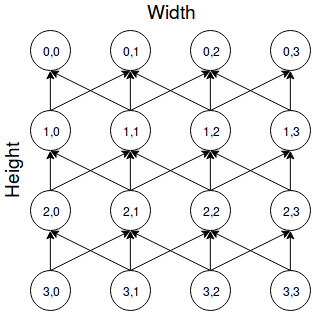
\includegraphics[scale=0.5]{GrapheSeamCarving.png}
   \end{figure}
\subsection{Algorithme des fonctions de coût}
\subsubsection{Comic}La fonction \textbf{ c(image,i,j)} permet de calculer la disposition minimale ainsi que son cout. Pour réduire les temps de calcul, cette fonction utilise la mémoïsation afin de sauvegarder la différence de largeur entre un ensemble d'images et la largeur souhaitée. Ceci ce fait en utilisant un tableau à deux dimensions (\textbf{memo} de taille $n \times n$). La sauvegarde se fait à l'intérieur de la fonction \textbf{cost(i,j,width)}.

Les résultats de découpe se fond dans la tableau \textbf{cuts}.
\begin{lstlisting}[frame=single]
c (image, i, j, memo, cuts)
	if(i>=j)
	{
		ADD i to cuts
		return cost(j,j), memo, cuts 
	}
	else
	{
		k=i
		while(true)
		{
			tmp=cost(k,j)
			if(tmp>cost(k+1,j,memo)
				k++
			else
				ADD k to cuts
				tmp += c(image, k, j, memo, cuts)
				break
		}
		return tmp, memo, cuts
	}
\end{lstlisting}
\subsubsection{Seam carving}
La fonction\textbf{ E(image,i,j)} est la fonction qui calcule l'énergie d'un pixel. Le tableau \textbf{energies} contient les coutures d'énergie minimales pour atteindre chaque pixel depuis la première rangée. Le tableau \textbf{moves} contient le déplacement à faire (gauche, centre, droite) pour suivre une couture de bas en haut. 
\begin{lstlisting}[frame=single]
C (image, energies, moves)
for i=0 to n
	for j=0 to m
	{
	if i==0
		energies[i,j]=E(image,i,j)
	else
		if E(image,i-1,j-1) < E(image,i-1,j)
			tmp=E(image,i-1,j-1)
		else
			tmp=E(image,i-1,j)
		if tmp < E(image,i-1,j+1)
			min=tmp
		else
			min=E(image,i-1,j+1)
		energies[i,j]=E(image,i,j)+min
		if min == E(image,i-1,j-1)			
			moves[i,j]= -1
		else if min = E(image,i-1,j)
			moves[i,j]=0
		else
			moves[i,j]=1
	}
return energies, moves
\end{lstlisting}

\subsection{Complexité en temps et en espace}
\subsubsection{Comic}
La complexité en temps de l'algorithme est $\Theta(n)$. La fonction \textbf{cost()} peut potentiellement ralentir l'exécution sa complexité est $O(\frac{n^2}{2})$ dans le pire des cas.
La complexité en espace est $\Theta(n \times (n+2))$. Les images, le tableau $n^2$ pour la mémoïsation et un tableau de découpe de taille $n$.
\subsubsection{Seam carving}
La complexité en temps de l'algorithme est $\Theta(n*m)$
La complexité en espace est $\Theta(3*n*m)$. Car il y a trois tableaux de dimension n*m. L'image en elle même, plus un tableau pour enregistrer les coutures d'énergie et un tableau pour enregistrer les déplacements à faire pour suivre une couture de bas en haut.

\section{Fonctions de réduction et d'augmentation d'images}
\subsection{Choix d'implémentation}
Les deux fonctions \textbf{ImageWidthReduction} et \textbf{ImageWidthexpansion} sont très proches dans leur fonctionnement. La seule différence est lorsqu'on crée une nouvelle image temporaire, respectivement plus grande ou plus petite de 1 pixel.

Une fonction \textbf{energie} renvoie l'énergie calculée d'un pixel donné en argument avec l'image auquel il appartient.

La fonction \textbf{seams} utilise la fonction \textbf{energie} pour remplir le tableau contenant les coutures d'énergie minimales pour chaque pixel de l'image transmise en argument. Elle remplit également le tableau indiquant les déplacements à effectuer pour suivre les coutures minimales depuis la dernière ligne de l'image.

La fonction \textbf{selectedSeam} parcourt le tableau  des coutures pour enregistrer le numéro de colonne de chaque pixel de la couture minimale dans un vecteur de taille correspondant à la hauteur de l'image. 

Les opérations décrites ci-dessous sont effectuées un nombre de fois correspondant au nombre de pixels que l'on souhaite ajouter ou diminuer sur la largeur de l'image.

Au sein des fonctions \textbf{ImageWidthReduction} et \textbf{ImageWidthexpansion}, pour chaque iteration, on sélectionne la couture d'énergie minimale au moyen des fonctions décrites ci-dessus. Ensuite, pour générer une nouvelle image de largeur +/- 1 à chaque iteration, on travaille avec deux pointeurs vers deux images temporaires. L'image pointée par "new" est initialement de la même taille que l'image originelle. L'image pointée par "tmp" est l'image augmentée ou réduite d'un pixel en largeur par rapport à new. Lorsqu'une couture est sélectionnée sur l'image de "new", l'image de "tmp" est construite en tenant compte de la couture. Ensuite, l'image pointée par "new" est détruite, et "new" pointe vers l'image de "tmp". A l'itération suivante, "tmp" pointe vers une nouvelle image, plus petite ou plus grande que "new".

\subsection{Complexité en temps et en espace}
Les complexités en temps et en espace sont identiques pour les deux fonctions.
\subsubsection{Complexité en espace}
	En plus de l'image originelle, deux autres images avec un écart de largeur égal à 1 sont générées pour les calculs. En fonction des itérations, leur largeur évolue entre la largeur originelle et la largeur cible. A ces deux images s'ajoutent le tableau contenant les coutures et le tableau contenant les déplacements. Les largeurs des deux tableaux évoluent comme les images. Et à cela s'ajoute un vecteur de taille "n", contenant les numéros de colonne des pixels impliqués dans la couture sélectionnée.
	La complexité en espace est donc maximale au début de la fonction : $\theta(3*(n*m) + n*(m-1) + n)$ = $\theta(4*n*m)$
\subsubsection{Complexité en temps}
	Pour diminuer ou augmenter une image de 1px en largeur la complexité en temps est la suivante :
L'image est parcourue une fois pour déterminer les coutures($\theta(n*m)$). Elle est ensuite parcourue en largeur et en hauteur pour déterminer la couture d'énergie minimale ($\theta(n+m)$). L'image est ensuite parcourue une nouvelle fois pour générer une nouvelle image. Là la complexité change en fonction de si l'on veut agrandir ou rétrécir l'image :
\begin{itemize}
 \item Agrandir : une colonne en plus est générée ($\theta(n*m + n)$). On a donc au total une complexité $\theta(2n*m + m + 2n)$
 \item Rétrécir : une colonne en moins est parcourue ($\theta(n*m - n)$). On a donc au total une complexité $\theta(2n*m + m)$
 \end{itemize}
 Il faut maintenant prendre en compte le nombre k d'itérations à effectuer pour modifier l'image de k pixels en largeur. En faisant attention que la taille des tableaux diminue à chaque itération
 
\textbf{Rétrécissement d'une image:}
$$
 	T_{n,m,k} = \sum\limits_{i=0}^{k} 2n(m-i) + m-i 
$$
$$
 	= (2n + 1)\sum\limits_{i=0}^{k} (m -i)
$$
$$
 	= (2n + 1)(\sum\limits_{i=0}^{k} m - \sum\limits_{i=0}^{k} i)
$$
$$
 	= (2n + 1)(k*m - \frac{k(k+1)}{2})
$$
$$
 	= k(2n + 1)(m - \frac{(k+1)}{2})
$$
Lorsque k est négligeable par rapport à m, la complexité est proche de $\theta(2knm)$\\
\textbf{Agrandissement d'une image:} \\
En s'aidant de la formule précédente, on arrive facilement à la formule suivante :
$$
 	T_{n,m,k} = (2n + 1)\sum\limits_{i=0}^{k} (m -i) + \sum\limits_{i=0}^{k} 2n
$$
$$
 	= k2n + k(2n + 1)(m - \frac{(k+1)}{2})
$$
Encore une fois, lorsque k est négligeable par rapport à m, et en prenant en compte que $k2n$ est négligeable par rapport au reste de la formule, on a une complexité proche de $\theta(2knm)$ 
 
\end{document}
